\chapter{Energy, Inner Products, and Hermiticity}
\label{ch:energy-inner}

\begin{chapterlead}
Before we can say what non-Hermitian photonics \emph{is}~\cite{ozawa2018topological,bergholtz2019exceptional}, we must understand
what it \emph{is not}. The entire machinery of lossless electromagnetism---real
eigenfrequencies, orthogonal modes, energy conservation, reciprocity---rests
on a single mathematical fact: the Maxwell curl--curl operator is self-adjoint
with respect to an energy inner product. That inner product is derived
from the Poynting theorem, leading to the self-adjointness conditions
and catalogs the physical mechanisms that destroy them. Every later chapter
of this book is, in one way or another, a study of the consequences of that
destruction.
\end{chapterlead}


%% ================================================================
\section{Poynting's theorem}
\label{sec:poynting}

We begin, as always, from Maxwell's equations. Taking the dot product of
Faraday's law~\eqref{eq:faraday} with $\HH$ and of Amp\`ere's
law~\eqref{eq:ampere} with $\EE$, and subtracting, one obtains the
\emph{Poynting identity} in its instantaneous, differential form:
\begin{equation}
 \boxed{
 \divg\mathbf{S}
 = -\EE\cdot\pdv{\DD}{t} - \HH\cdot\pdv{\BB}{t},
 }
 \label{eq:poynting-diff}
\end{equation}
where the Poynting vector is
\begin{equation}
 \mathbf{S} = \EE\times\HH,
 \label{eq:poynting-vector}
\end{equation}
At this stage, \eqref{eq:poynting-diff} is only an identity: it follows
from Maxwell's equations alone and makes no assumption about the
constitutive relations. An energy density appears only after the material
response is specified well enough that
$\EE\cdot\partial_t\DD+\HH\cdot\partial_t\BB$ can be written as a total
time derivative.

For a \emph{nondispersive, lossless} medium with real, frequency-independent
$\epsr(\rr)$ and $\mur(\rr)$, the right-hand side simplifies:
\begin{equation}
 \EE\cdot\pdv{\DD}{t} + \HH\cdot\pdv{\BB}{t}
 = \pdv{}{t}\!\left[
 \frac{1}{2}\epsvac\epsr|\EE|^2
 + \frac{1}{2}\muvac\mur|\HH|^2
 \right].
 \label{eq:u-nondispersive}
\end{equation}
The energy density is therefore
\begin{equation}
 u(\rr,t) = \frac{1}{2}\epsvac\epsr(\rr)\,|\EE(\rr,t)|^2
 + \frac{1}{2}\muvac\mur(\rr)\,|\HH(\rr,t)|^2,
 \label{eq:energy-density}
\end{equation}
and the Poynting theorem becomes a local conservation law:
\begin{equation}
 \pdv{u}{t} + \divg\mathbf{S} = 0.
 \label{eq:energy-conservation}
\end{equation}
Integrating over a volume $\Omega$ bounded by a surface $\partial\Omega$,
\begin{equation}
 \dv{}{t}\int_\Omega u\;\dd^3 r
 = -\oint_{\partial\Omega}\mathbf{S}\cdot\nn\;\dd S.
 \label{eq:energy-integral}
\end{equation}
The total electromagnetic energy in $\Omega$ changes only through the Poynting
flux through its boundary. No energy is created or destroyed inside the
volume. This is the physical content of ``lossless'': energy is a
conserved quantity.

\paragraph{Example: energy balance in a lossy dielectric slab.}
Consider a plane wave $\EE = E_0\,e^{i(kz-\omega t)}\hat{\mathbf{x}}$
propagating in a slab of thickness $d$ with complex permittivity
$\epsr = \epsr' + i\epsr''$. To isolate absorption from interface
reflection, take $E_0$ below to denote the forward field just inside an
impedance-matched slab. The time-averaged Poynting flux entering the
material is then $S_{\mathrm{in}} = |E_0|^2/(2\eta)$, where
$\eta = \sqrt{\muvac/(\epsvac\epsr')}$ in the weak-loss limit.
Inside the slab, the field decays approximately as
$|\EE(z)|^2 = |E_0|^2 e^{-2\alpha z}$, where the attenuation constant
is $\alpha = (\omega/c)\Im\sqrt{\epsr}$. The time-averaged dissipated
power per unit area is
\begin{equation}
 P_{\mathrm{diss}} = \frac{\omega\epsvac\epsr''}{2}
 \int_0^d |E_0|^2 e^{-2\alpha z}\;\dd z
 = \frac{\omega\epsvac\epsr''\,|E_0|^2}{4\alpha}
 \bigl(1 - e^{-2\alpha d}\bigr).
 \label{eq:slab-dissipation}
\end{equation}
The Poynting flux exiting the slab is
$S_{\mathrm{out}} = S_{\mathrm{in}}\,e^{-2\alpha d}$ in the same weak-loss
description. Equivalently, the local identity
$-\mathrm{d}S/\mathrm{d}z =
(\omega\epsvac\epsr''/2)|E(z)|^2$ gives
$S_{\mathrm{in}} - S_{\mathrm{out}} = P_{\mathrm{diss}}$: the energy
lost from the wave equals the energy absorbed by the medium. With
interfaces included, reflected fluxes must also be counted, but the same
Poynting balance holds exactly.

When $\epsr'' < 0$ (gain medium), $\alpha < 0$ and the field grows
exponentially. The ``dissipated'' power is negative---the medium
delivers energy to the wave. The Poynting flux \emph{increases}
across the slab, and $S_{\mathrm{out}} > S_{\mathrm{in}}$. This
simple example illustrates the core physical mechanism behind all
non-Hermitian photonic phenomena: the energy inner product is no
longer conserved when $\epsr'' \neq 0$.

Figure~\ref{fig:ch2-poynting-slab} illustrates this energy balance for
two independent slabs.

\begin{figure}[t]
 \centering
 
\includegraphics[width=0.95\linewidth]{fig_f2_poynting_slab_balance.pdf}
 \caption{Normalised Poynting flux $S(z)/S_{\mathrm{in}}$ through two
 independent dielectric slabs on separate vertical scales.
 (a)~Lossy slab ($\epsr''>0$): the flux decays exponentially from
 $S_{\mathrm{in}}=1$ to $S_{\mathrm{out}}=0.10$, so the medium
 absorbs $\Delta S/S_{\mathrm{in}}=0.90$. The sign convention
 $q=-\mathrm{d}S/\mathrm{d}z>0$ confirms that power density flows
 from the field into the material.
 (b)~Gain slab ($\epsr''<0$): the flux grows to
 $S_{\mathrm{out}}=3.00$, so the medium supplies
 $\Delta S/S_{\mathrm{in}}=2.00$ to the wave, with
 $q=-\mathrm{d}S/\mathrm{d}z<0$. In both panels, the dashed line
 marks $S_{\mathrm{in}}=1$ and the arrow at $z=d$ indicates the
 total flux change. The energy balance
 $S_{\mathrm{in}}-S_{\mathrm{out}}=\int_0^d q\,\mathrm{d}z$ is exact
 and follows directly from Poynting's theorem~\eqref{eq:poynting-diff}.}
 \label{fig:ch2-poynting-slab}
\end{figure}

\begin{booknote}[Units and conventions]
SI units are used throughout. The vacuum permittivity $\epsvac$ and
permeability $\muvac$ appear explicitly, so that $\epsr$ and $\mur$ are
dimensionless. The time convention is $e^{-i\omega t}$ for harmonic
fields. With this convention, a passive lossy medium has
$\Im\epsr(\omega) > 0$.
\end{booknote}


%% ================================================================
\section{Time-averaged energy and the harmonic inner product}
\label{sec:time-averaged}

For monochromatic fields with harmonic time dependence
$\EE(\rr,t) = \Re[\EE(\rr)\,e^{-i\omega t}]$, the time-averaged energy
density is
\begin{equation}
 \langle u \rangle
 = \frac{1}{4}\epsvac\epsr(\rr)\,|\EE(\rr)|^2
 + \frac{1}{4}\muvac\mur(\rr)\,|\HH(\rr)|^2,
 \label{eq:time-avg-u}
\end{equation}
and the time-averaged Poynting vector is
\begin{equation}
 \langle\mathbf{S}\rangle
 = \frac{1}{2}\Re\!\bigl[\EE(\rr)\times\HH^*(\rr)\bigr].
 \label{eq:time-avg-S}
\end{equation}

These expressions are valid only when $\epsr$ and $\mur$ are real and
frequency-independent. For dispersive media, additional terms involving
$\dd\epsr/\dd\omega$ appear (the Brillouin formula), and for lossy media,
the time-averaged ``energy density'' is no longer uniquely defined from
the macroscopic fields alone---a point we shall return to in
Chapter~\ref{ch:loss-gain-dispersion}.

The positive-definiteness of $\langle u\rangle$ when $\epsr > 0$ and
$\mur > 0$ is crucial. It means that the electromagnetic energy defines a
norm on the space of field configurations, and hence an inner product.


%% ================================================================
\section{Inner products for the Maxwell eigenproblem}
\label{sec:inner-products}

The eigenvalue problems derived in Chapter~\ref{ch:light-eigenvalue} have
natural inner products dictated by the energy density.

\subsection{The $\HH$-field inner product}
\label{ssec:H-inner}

For the operator $\Mop$ defined in~\eqref{eq:maxwell-op-H}, the natural
inner product is
\begin{equation}
 \langle\HH_1,\,\HH_2\rangle
 = \int_\Omega \HH_1^*(\rr)\cdot\HH_2(\rr)\;\dd^3 r.
 \label{eq:H-inner}
\end{equation}
This is the standard $L^2$ inner product, unweighted, because the
eigenvalue equation $\Mop\HH = (\omega^2/c^2)\HH$ has the eigenvalue on
the right without a material weight (assuming $\mur = 1$).

\subsection{The $\EE$-field inner product}
\label{ssec:E-inner}

For the $\EE$-field equation~\eqref{eq:curlcurl-E}, the eigenvalue appears
multiplied by $\epsr(\rr)$, so the correct inner product is the
$\epsr$-weighted one introduced in \eqref{eq:inner-product}:
\begin{equation}
 \langle\EE_1,\,\EE_2\rangle_\eps
 = \int_\Omega \EE_1^*(\rr)\cdot\epsr(\rr)\,\EE_2(\rr)\;\dd^3 r.
 \label{eq:E-inner-repeat}
\end{equation}
This inner product is positive-definite precisely when $\epsr(\rr) > 0$
for scalar media, or when the permittivity tensor is Hermitian positive
definite in anisotropic media.

\begin{figure}[t]
 \centering
 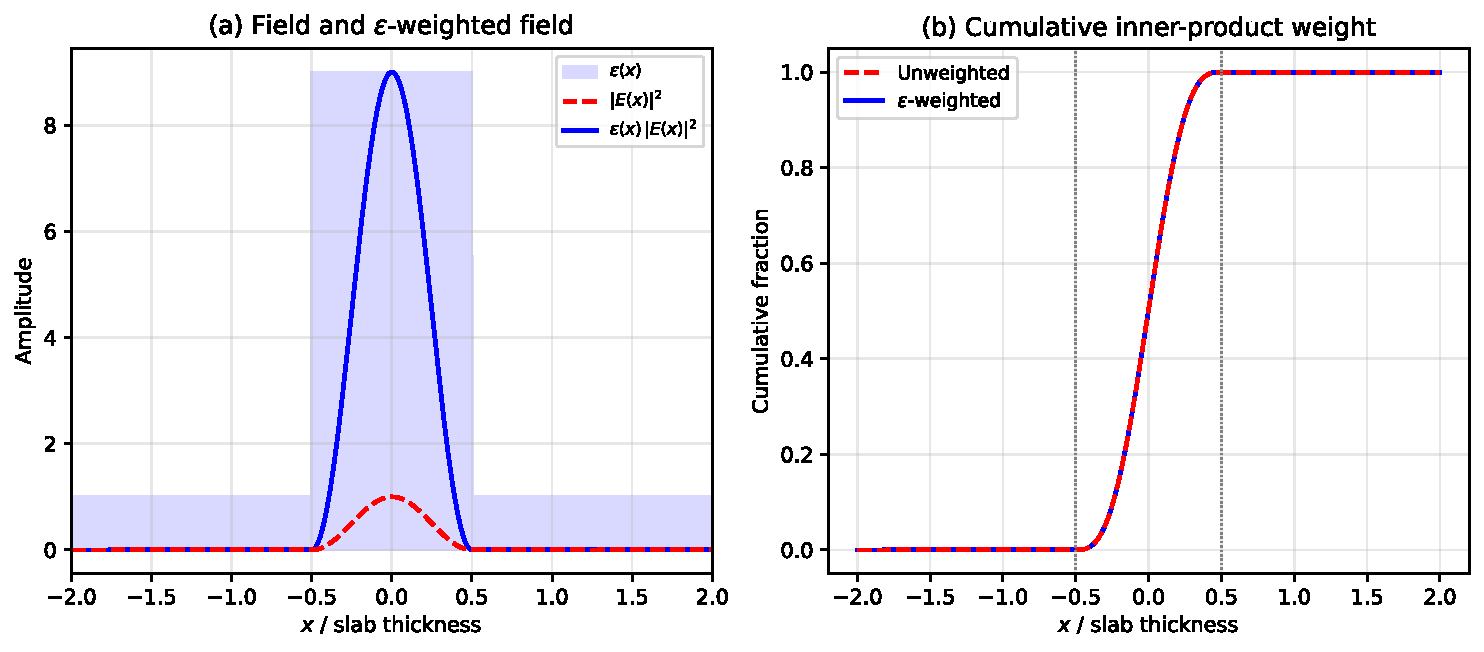
\includegraphics[width=0.85\linewidth]{figures/fig_f02_inner_product_weight.pdf}
 \caption{Visualisation of the $\varepsilon$-weighted inner product for
 a dielectric slab ($\varepsilon = 9$, shaded region).
 (a)~The bare field intensity $|E(x)|^2$ (red) and the
 $\varepsilon$-weighted intensity $\varepsilon(x)\,|E(x)|^2$ (blue).
 The weighting amplifies the contribution from the high-index region,
 reflecting the physical energy density $\frac{1}{2}\varepsilon_0
 \varepsilon|E|^2$.
 (b)~Cumulative inner-product weight: the $\varepsilon$-weighted
 curve (solid blue) rises steeply inside the slab, showing that most
 of the modal energy resides in the high-index material.}
 \label{fig:inner-product-weight}
\end{figure}


\subsection{The first-order Maxwell inner product}
\label{ssec:first-order-inner}

There is a third, often more natural, way to organize the Maxwell
eigenproblem. Writing the six-component field vector
$\mathbf{\Psi} = (\EE,\,\HH)^\transpose$,
the frequency-domain Maxwell equations~\eqref{eq:faraday-freq}--\eqref{eq:ampere-freq}
become a first-order system
\begin{equation}
 \underbrace{
 \begin{pmatrix}
 0 & i\curl \\[3pt]
 -i\curl & 0
 \end{pmatrix}
 }_{\displaystyle\hat{\mathcal{M}}}
 \begin{pmatrix} \EE \\ \HH \end{pmatrix}
 = \omega
 \underbrace{
 \begin{pmatrix}
 \epsvac\epsr & 0 \\[3pt]
 0 & \muvac\mur
 \end{pmatrix}
 }_{\displaystyle\hat{W}}
 \begin{pmatrix} \EE \\ \HH \end{pmatrix}.
 \label{eq:first-order-maxwell}
\end{equation}
The operator $\hat{\mathcal{M}}$ is manifestly Hermitian with respect to
the unweighted $L^2$ inner product (its off-diagonal blocks are related
by the curl identity~\eqref{eq:curl-ibp}). The generalized eigenvalue
problem $\hat{\mathcal{M}}\mathbf{\Psi} = \omega\,\hat{W}\mathbf{\Psi}$
is self-adjoint with respect to the energy inner product
\begin{equation}
 \langle\mathbf{\Psi}_1,\,\mathbf{\Psi}_2\rangle_W
 = \int_\Omega \mathbf{\Psi}_1^\adj\,\hat{W}\,\mathbf{\Psi}_2\;\dd^3 r
 = \int_\Omega\!\bigl[
 \epsvac\epsr\,\EE_1^*\cdot\EE_2
 + \muvac\mur\,\HH_1^*\cdot\HH_2
 \bigr]\dd^3 r,
 \label{eq:energy-inner-full}
\end{equation}
provided $\epsr$ and $\mur$ are real and positive and the boundary
conditions make the surface terms vanish. This inner product is
proportional to four times the time-averaged electromagnetic energy when
$\mathbf{\Psi}_1 = \mathbf{\Psi}_2$.

\paragraph{Comparing the three inner products on a concrete mode pair.}
To see how the three inner products differ in practice, consider the
fundamental TE$_{10}$ and TE$_{01}$ modes of a rectangular metallic
cavity ($a \times b \times d$) filled with a uniform dielectric
$\epsr = \mathrm{const}$, $\mur = 1$. The $\HH$-fields of these two
modes are $\HH_1 = H_0\cos(\pi x/a)\sin(\pi z/d)\,\hat{\mathbf{y}}$ and
$\HH_2 = H_0\sin(\pi y/b)\cos(\pi z/d)\,\hat{\mathbf{x}}$ (simplified for
illustration). The three inner products give:
\begin{enumerate}
 \item $\langle\HH_1,\HH_2\rangle = \int \HH_1^*\cdot\HH_2\;\dd^3r
 = 0$, because $\hat{\mathbf{x}}\cdot\hat{\mathbf{y}} = 0$ (orthogonal
 polarizations).
 \item $\langle\EE_1,\EE_2\rangle_\eps
 = \int \epsr\,\EE_1^*\cdot\EE_2\;\dd^3r = 0$, because the
 $\EE$-fields of the two modes have different spatial symmetries
 under the cavity's $C_{2v}$ group.
 \item $\langle\mathbf{\Psi}_1,\mathbf{\Psi}_2\rangle_W
 = \int(\epsvac\epsr\,\EE_1^*\cdot\EE_2
 + \muvac\,\HH_1^*\cdot\HH_2)\;\dd^3r = 0$, as both terms vanish
 independently.
\end{enumerate}
All three inner products agree (zero) for this mode pair in the
Hermitian case. The distinction matters only when $\epsr$ is complex
or when the modes are quasinormal: then the $\HH$-field inner product
stays unchanged (it does not involve $\epsr$), the $\EE$-field inner
product picks up an imaginary contribution from $\epsr''$, and the
first-order inner product mixes both. In non-Hermitian photonics~\cite{kawabata2018symmetry}, the
choice of inner product is not a convention but a physical decision
that determines orthogonality, completeness, and the meaning of
``energy.''

\begin{takeaway}[Energy as inner product]
The electromagnetic energy density defines the inner product that makes
the Maxwell operator self-adjoint. Making $\epsr$ complex, opening the
boundary, or projecting onto a subspace changes this inner product and
therefore changes the adjointness properties of the problem.
\end{takeaway}


%% ================================================================
\section{Self-adjointness: the complete argument}
\label{sec:self-adjoint-proof}

We now give a careful derivation of the self-adjointness of $\Mop$ in the
$\HH$-field formulation~\eqref{eq:maxwell-op-H}, which was stated without
full proof in Section~\ref{sec:self-adjoint}.

\begin{theorem}[Self-adjointness of $\Mop$]
\label{thm:self-adjoint}
Let $\Omega$ be a domain in $\mathbb{R}^3$ with piecewise smooth boundary
$\partial\Omega$. Let $\epsr(\rr)$ be real, positive, and bounded away
from zero, and let $\mur = 1$. Define
$\Mop\HH = \curl[\epsr^{-1}\curl\HH]$. Then $\Mop$ is self-adjoint with
respect to $\langle\cdot,\cdot\rangle$ on the space of divergence-free
fields satisfying either
(a)~$\nn\times\EE = 0$ on $\partial\Omega$ (perfect electric conductor),
or (b)~Bloch-periodic boundary conditions.
\end{theorem}

\begin{proof}
Consider two fields $\HH_1$ and $\HH_2$ in the domain of $\Mop$. We
compute
\begin{align}
 \langle\HH_1,\,\Mop\HH_2\rangle
 &= \int_\Omega \HH_1^*\cdot
 \curl\!\bigl[\epsr^{-1}\curl\HH_2\bigr]\;\dd^3 r.
 \label{eq:sa-step1}
\end{align}
Using the vector identity
$\mathbf{A}\cdot(\curl\mathbf{B})
 = (\curl\mathbf{A})\cdot\mathbf{B}
 + \divg(\mathbf{B}\times\mathbf{A})$
with $\mathbf{A} = \HH_1^*$ and
$\mathbf{B} = \epsr^{-1}\curl\HH_2$, we obtain
\begin{equation}
 \langle\HH_1,\,\Mop\HH_2\rangle
 = \int_\Omega \frac{1}{\epsr}\,
 (\curl\HH_1)^*\cdot(\curl\HH_2)\;\dd^3 r
 + \oint_{\partial\Omega}
 \bigl(\epsr^{-1}\curl\HH_2\times\HH_1^*\bigr)\cdot\nn\;\dd S.
 \label{eq:sa-step2}
\end{equation}
The bulk integral on the right is manifestly symmetric under the exchange
$1\leftrightarrow 2$ (with complex conjugation), because $\epsr^{-1}$ is
real. The surface integral vanishes under either boundary condition~(a)
or~(b).

For condition~(a), note that $\epsr^{-1}\curl\HH = (i\omega\epsvac)^{-1}\EE$
from Amp\`ere's law, so
$\nn\times(\epsr^{-1}\curl\HH) \propto \nn\times\EE = 0$
on $\partial\Omega$.

For condition~(b), the integrand on opposite faces of the unit cell
differs by Bloch phases $e^{i\kk\cdot\mathbf{a}}$ and $e^{-i\kk\cdot\mathbf{a}}$,
while the outward normals are opposite; the contributions cancel.

Since the bulk term is symmetric and the surface term vanishes,
\begin{equation}
 \langle\HH_1,\,\Mop\HH_2\rangle
 = \langle\Mop\HH_1,\,\HH_2\rangle,
 \label{eq:sa-result}
\end{equation}
completing the proof.
\end{proof}

The same argument can be repeated for the $\EE$-field
operator with the $\epsr$-weighted inner product, yielding
$\langle\EE_1,\,\Mop_E\EE_2\rangle_\eps
 = \langle\Mop_E\EE_1,\,\EE_2\rangle_\eps$
under the same boundary conditions.

\begin{remark}
The assumption that $\epsr$ is real enters at a precise point: the
symmetry of the bulk integral in~\eqref{eq:sa-step2}. If
$\epsr = \epsr' + i\epsr''$ with $\epsr'' \neq 0$, then
$1/\epsr^* \neq 1/\epsr$, the bulk term is no longer symmetric,
and self-adjointness fails. This is the mathematical origin of
non-Hermiticity from material loss or gain.
\end{remark}


%% ================================================================
\section{Consequences of self-adjointness}
\label{sec:sa-consequences}

When $\Mop$ is self-adjoint, the standard theorems of spectral theory for
compact self-adjoint operators in a Hilbert space apply. The consequences
are profound and familiar, but it is worth stating them explicitly, because
each one can fail in non-Hermitian photonics.

\subsection{Real eigenvalues}
\label{ssec:real-eigenvalues}

If $\Mop\HH_n = \lambda_n\HH_n$ with $\lambda_n = \omega_n^2/c^2$, then
\begin{equation}
 \lambda_n = \frac{\langle\HH_n,\,\Mop\HH_n\rangle}
 {\langle\HH_n,\,\HH_n\rangle}
 = \frac{\displaystyle\int_\Omega\epsr^{-1}|\curl\HH_n|^2\;\dd^3 r}
 {\displaystyle\int_\Omega|\HH_n|^2\;\dd^3 r}
 \;\ge\; 0.
 \label{eq:rayleigh-quotient}
\end{equation}
The eigenvalue $\lambda_n$ is real and non-negative: the eigenfrequencies
$\omega_n$ are real. There is no temporal decay, no growth, no complex
frequency.

\subsection{Orthogonality}
\label{ssec:orthogonality}

Eigenmodes belonging to distinct eigenvalues are orthogonal:
\begin{equation}
 \omega_m \neq \omega_n
 \quad\Longrightarrow\quad
 \langle\HH_m,\,\HH_n\rangle = 0.
 \label{eq:orthogonality}
\end{equation}
For the $\EE$-field formulation, the orthogonality relation is
$\langle\EE_m,\,\EE_n\rangle_\eps = 0$.

In either case, we may normalize the modes so that
$\langle\HH_m,\,\HH_n\rangle = \delta_{mn}$ or
$\langle\EE_m,\,\EE_n\rangle_\eps = \delta_{mn}$. Mode decompositions
and projections are then uniquely defined.

\subsection{Completeness}
\label{ssec:completeness}

For a compact domain (closed cavity), the eigenmodes form a complete
orthonormal basis. Any field satisfying the boundary conditions can be
expanded:
\begin{equation}
 \HH(\rr) = \sum_n c_n\,\HH_n(\rr),
 \qquad
 c_n = \langle\HH_n,\,\HH\rangle.
 \label{eq:completeness}
\end{equation}
The expansion coefficients $c_n$ are uniquely determined by the inner
product, and Parseval's identity
$\|\HH\|^2 = \sum_n |c_n|^2$ holds.

\subsection{Variational characterization}
\label{ssec:variational}

The eigenfrequencies can be obtained from the Rayleigh quotient:
\begin{equation}
 \omega_1^2/c^2
 = \min_{\HH\neq 0}\;
 \frac{\displaystyle\int\epsr^{-1}|\curl\HH|^2\;\dd^3 r}
 {\displaystyle\int|\HH|^2\;\dd^3 r},
 \label{eq:variational}
\end{equation}
with higher eigenvalues given by the min--max principle. This
characterization is the basis of numerical methods such as the plane-wave
expansion and finite-element eigensolvers used in photonic-crystal
computations~\cite{paz2019tutorial}.


%% ================================================================
\section{Lorentz reciprocity}
\label{sec:reciprocity}

Self-adjointness (Hermiticity) is not the only symmetry of the Maxwell
operator. There is a distinct and equally important property:
\emph{reciprocity}.

Consider two source--field pairs $(\JJ_a, \EE_a, \HH_a)$ and
$(\JJ_b, \EE_b, \HH_b)$ at the same frequency $\omega$ in a medium
with $\epsr(\rr)$ and $\mur(\rr)$ that are symmetric tensors (which
includes all isotropic and many anisotropic media). The Lorentz
reciprocity theorem states
\begin{equation}
 \int_\Omega\bigl(\EE_a\cdot\JJ_b - \EE_b\cdot\JJ_a\bigr)\;\dd^3 r
 = \oint_{\partial\Omega}
 \bigl(\EE_a\times\HH_b - \EE_b\times\HH_a\bigr)\cdot\nn\;\dd S.
 \label{eq:lorentz-reciprocity}
\end{equation}
If the surface integral vanishes (closed cavity, or sources far from
$\partial\Omega$), this reduces to the familiar statement
$\langle\EE_a,\JJ_b\rangle = \langle\EE_b,\JJ_a\rangle$:
swapping source and observation gives the same field projection.

\subsection{Reciprocity and the scattering matrix}
\label{ssec:reciprocity-smatrix}

Reciprocity has a direct and powerful consequence for the scattering
matrix $S(\omega)$ of Chapter~\ref{ch:boundaries}. If the medium is
reciprocal (symmetric $\epsr$ and $\mur$ tensors), then the $S$-matrix
satisfies
\begin{equation}
 S^\transpose(\omega) = S(\omega),
 \label{eq:s-reciprocity}
\end{equation}
i.e., $S$ is a symmetric matrix. This means that the transmission from
port $i$ to port $j$ equals the transmission from port $j$ to port $i$:
$S_{ij} = S_{ji}$.

The proof follows from the Lorentz reciprocity
theorem~\eqref{eq:lorentz-reciprocity}. Let $\EE_a$ be the field
produced by a source at port~$i$ and $\EE_b$ the field from a source at
port~$j$. If the surface integral vanishes (all ports are included in
the integration surface), then
$\langle\EE_a,\JJ_b\rangle = \langle\EE_b,\JJ_a\rangle$, which
translates directly into $S_{ij} = S_{ji}$ when expressed in the
scattering-matrix language.

This symmetry is \emph{not} the same as unitarity. A unitary $S$-matrix
($S^\dagger S = I$) expresses energy conservation and requires
Hermiticity; a symmetric $S$-matrix ($S^\transpose = S$) expresses
reciprocity and requires only symmetric material tensors. A lossy
dielectric cavity has $S^\transpose = S$ (reciprocal) but
$S^\dagger S \neq I$ (energy is absorbed). A magneto-optic material
breaks the tensor symmetry and therefore breaks both reciprocity and
$S$-matrix symmetry, even if the system is lossless.

The distinction between reciprocity (symmetric $S$) and Hermiticity
(unitary $S$) is the scattering-theory counterpart of the distinction
between the unconjugated bilinear form and the conjugate inner product
in the operator formulation.

\begin{booknote}[Reciprocity versus Hermiticity]
Reciprocity and Hermiticity are conceptually distinct.
\emph{Hermiticity} involves the complex-conjugate inner product
$\langle\mathbf{F}^*,\Mop\mathbf{G}\rangle$ and requires $\epsr$ to be
\emph{real}. \emph{Reciprocity} involves an unconjugated bilinear form
$(\mathbf{F},\sigma\mathbf{G})$ and requires $\epsr$ to be a
\emph{symmetric tensor}. A medium with complex $\epsr = \epsr' + i\epsr''$
that is scalar (or symmetric) is \emph{reciprocal but not Hermitian}.
This distinction is central to non-Hermitian photonics: many systems of
interest---lossy dielectrics, gain media, $\PT$-symmetric
structures---are reciprocal, even though they are not Hermitian.
The reaction-based inner product exploited in coupled-mode
theory~\cite{xu2015general} is built on reciprocity, not Hermiticity.
\end{booknote}


%% ================================================================
\section{Four roads to non-Hermiticity}
\label{sec:four-roads}

The self-adjointness proof of Section~\ref{sec:self-adjoint-proof} relied on
three assumptions: (i)~$\epsr$ real, (ii)~boundary terms vanish,
(iii)~fields live in a complete Hilbert space. The Rayleigh quotient
argument~\eqref{eq:rayleigh-quotient} additionally used $\epsr > 0$.
Violating any of these opens a distinct road to non-Hermitian physics.
Figure~\ref{fig:ch2-hermiticity-map} summarises the logical structure.

\begin{figure}[t]
 \centering
 
\includegraphics[width=0.92\linewidth]{fig_f2_hermiticity_conditions.pdf}
 \caption{Conditions for Maxwell self-adjointness and the four common
 mechanisms that break them.
 (a)~Three sufficient conditions---positive Hermitian constitutive
 tensors $\varepsilon,\mu$, vanishing boundary flux (closed domain),
 and a complete Hilbert space---ensure that the Maxwell curl-curl
 operator is self-adjoint in the energy inner product, yielding a
 real spectrum, orthogonal modes, and conserved electromagnetic
 energy.
 (b)~Each condition can be violated independently: material loss or
 gain introduces complex $\varepsilon$; radiation through open
 boundaries allows energy to leave the domain; frequency-dependent
 $\varepsilon(\omega)$ makes the operator effectively non-self-adjoint
 at any fixed real frequency; and projection onto a finite mode
 subspace discards completeness. The resulting non-Hermitian
 spectra exhibit complex eigenfrequencies, non-orthogonal modes,
 exceptional points, and possible skin-effect localisation---the
 subjects of Parts~II--IV of this monograph.}
 \label{fig:ch2-hermiticity-map}
\end{figure}


\subsection{Material loss and gain}
\label{ssec:road-lossgain}

If the permittivity has an imaginary part, $\epsr = \epsr' + i\epsr''$, the
factor $\epsr^{-1}$ in~\eqref{eq:sa-step2} is no longer real, and the bulk
integral loses its symmetry. For monochromatic fields in a nondispersive
medium, the time-averaged Poynting identity becomes
\begin{equation}
 \divg\langle\mathbf{S}\rangle
 = -\frac{\omega}{2}\epsvac\epsr''(\rr)\,|\EE(\rr)|^2.
 \label{eq:poynting-lossy}
\end{equation}
For $\epsr'' > 0$ (our $e^{-i\omega t}$ convention), energy is absorbed;
for $\epsr'' < 0$, energy is emitted. The eigenfrequencies become complex,
and modes are no longer orthogonal with respect to
$\langle\cdot,\cdot\rangle_\eps$.

\paragraph{Physical example: coupled whispering-gallery resonators.}
Two silica microsphere resonators (diameter $\sim 50\;\mu$m) coupled
evanescently through a sub-wavelength air gap provide a clean realisation.
When both spheres are passive (intrinsic material loss only,
$\epsr'' \sim 10^{-7}$), the system is nearly Hermitian: the two
whispering-gallery modes split into symmetric and antisymmetric
supermodes with real frequency splitting $2\kappa$. When one sphere is
doped with an erbium gain medium pumped above threshold ($\epsr'' < 0$),
the system becomes genuinely non-Hermitian: the two supermodes acquire
different imaginary parts, and at a critical pump power the frequency
splitting vanishes at an exceptional point. The transition from the
Hermitian regime ($\epsr'' = 0$) to the EP ($|\epsr''|$ reaches the
critical value) is a continuous deformation of the eigenvalue structure
that can be tracked experimentally through the transmission spectrum.

This mechanism is explored in Chapter~\ref{ch:loss-gain-dispersion} and
provides the physical basis for $\PT$-symmetric optics
(Chapter~\ref{ch:pt-symmetric}).

\subsection{Radiation and open boundaries}
\label{ssec:road-radiation}

For an open system, the outgoing-wave (Sommerfeld) boundary condition
replaces the standing-wave condition of a closed cavity. The surface
integral in~\eqref{eq:sa-step2} no longer vanishes: energy flows outward
through $\partial\Omega$. As a result, eigenfrequencies acquire negative
imaginary parts (fields decay in time while growing spatially toward
infinity). These are the quasinormal modes of Chapter~\ref{ch:qnm}.

\paragraph{Physical example: a dielectric microsphere in vacuum.}
A dielectric sphere of radius $R$ and $\epsr = 4$ (e.g., a glass
microsphere) supports whispering-gallery modes with $Q$ factors that
increase exponentially with the angular momentum $\ell$. Each mode has
a complex eigenfrequency $\omega_\ell = \omega_\ell' - i\gamma_\ell/2$,
where $\gamma_\ell$ is the radiative decay rate. Even though the
material is perfectly lossless ($\epsr'' = 0$), the eigenfrequencies are
complex because the outgoing-wave boundary condition at $r \to \infty$
breaks the self-adjointness of the Maxwell operator. The non-Hermiticity
is purely geometrical: it arises from the open boundary, not from any
material dissipation.

\subsection{Frequency dispersion}
\label{ssec:road-dispersion}

Even for a closed, passive medium, if $\epsr(\omega)$ depends on frequency,
the eigenproblem is nonlinear in $\omega$ and the simple inner product
\eqref{eq:E-inner-repeat} is no longer the correct energy functional.
The Brillouin formula
\begin{equation}
 \langle u\rangle_{\mathrm{disp}}
 = \frac{1}{4}\epsvac\,
 \dv{}{\omega}\bigl[\omega\,\epsr'(\omega)\bigr]\,|\EE|^2
 + \frac{1}{4}\muvac\,
 \dv{}{\omega}\bigl[\omega\,\mur'(\omega)\bigr]\,|\HH|^2
 \label{eq:brillouin}
\end{equation}
gives a partial answer for weakly dispersive, low-loss media, but it is not
a true inner product: it is not bilinear, it depends on $\omega$, and it
becomes negative near absorption resonances. A rigorous treatment requires
auxiliary fields that restore the Hamiltonian structure of the dispersive
Maxwell system~\cite{figotin2004hamiltonian}. We defer this construction to
Chapter~\ref{ch:loss-gain-dispersion}, where it will be developed in detail.

\paragraph{Example: why the naive inner product fails for a
Lorentz medium.}
Consider a single Lorentz oscillator with permittivity
\begin{equation}
 \epsr(\omega) = 1 + \frac{\omega_p^2}{\omega_0^2 - \omega^2 - i\gamma\omega},
 \label{eq:lorentz-ch2}
\end{equation}
where $\omega_0$ is the resonance frequency, $\omega_p$ is the plasma
frequency, and $\gamma$ is the damping rate. At a frequency
$\omega$ well below the resonance ($\omega \ll \omega_0$), the
permittivity is approximately real and the naive inner product
$\langle \FF, \GG \rangle = \int \epsr\,\FF^* \cdot \GG\;\dd^3 r$ is
positive-definite. The Brillouin energy density~\eqref{eq:brillouin}
reduces to $\langle u \rangle_{\mathrm{disp}} \approx
\frac{1}{4}\epsvac\,(1 + \omega_p^2/\omega_0^2)\,|\EE|^2$, which is
the expected electrostatic energy enhanced by the polarizability.

Near the resonance ($\omega \approx \omega_0$), the situation changes
dramatically. The real part $\epsr'(\omega)$ passes through zero and
becomes negative, while the imaginary part $\epsr''(\omega)$ peaks at
$\omega_0$. The naive inner product is no longer positive-definite:
$\epsr'|\EE|^2$ can be negative, and the ``norm'' of a mode can
vanish or change sign. This is not a mathematical pathology but a
physical fact: near a material resonance, the electromagnetic energy is
stored partly in the kinetic energy of the polarization current, not
only in the field. The Brillouin formula accounts for this by
including the derivative $\partial(\omega\epsr')/\partial\omega$:
\begin{equation}
 \dv{}{\omega}\bigl[\omega\,\epsr'(\omega)\bigr]
 = 1 + \omega_p^2\,\frac{\omega_0^2 + \omega^2}
 {(\omega_0^2 - \omega^2)^2 + \gamma^2\omega^2},
 \label{eq:brillouin-derivative}
\end{equation}
which is positive for all $\omega$ when $\gamma$ is small (the
no-gain condition). The Brillouin energy thus remains positive even
where $\epsr'$ itself is negative---the ``missing'' energy is stored in
the oscillating polarization.

However, for $\gamma$ comparable to $\omega_0$ (strongly damped media),
the Brillouin formula itself becomes unreliable, and one must resort to
the auxiliary-field Hamiltonian embedding of
Chapter~\ref{ch:loss-gain-dispersion}, where the polarization degrees
of freedom are treated as dynamical variables on the same footing as the
electromagnetic field. This construction restores a true inner product
at the cost of enlarging the Hilbert space, and it is the key technical
step that makes the non-Hermitian Maxwell eigenproblem well-posed for
dispersive media.

\paragraph{Comparing inner products: lossless versus dispersive.}
The following table summarises the three regimes:
\begin{center}
\begin{tabular}{lcc}
 \hline
 \textbf{Regime} & \textbf{Weight} & \textbf{Positive-definite?} \\
 \hline
 Non-dispersive ($\epsr$ real, constant) &
 $\epsr\,|\EE|^2$ & Yes \\
 Weakly dispersive ($\gamma \ll \omega_0$) &
 $\partial_\omega(\omega\epsr')\,|\EE|^2$ & Yes \\
 Strongly dispersive ($\gamma \sim \omega_0$) &
 Auxiliary-field Hamiltonian & Yes (enlarged space) \\
 \hline
\end{tabular}
\end{center}
This table reflects the central message of Chapter~\ref{ch:energy-inner}:
as the medium becomes more realistic, the inner product that makes the
Maxwell operator self-adjoint becomes more complex, and the price of
restoring Hermiticity is paid either by restricting the frequency range
or by enlarging the state space.

\subsection{Projection onto a subspace}
\label{ssec:road-projection}

Even when the full Maxwell operator is self-adjoint, restricting attention
to a finite number of resonant modes creates an effective Hamiltonian that
is generically non-Hermitian. The discarded modes act as an environment:
they carry away energy (through radiation or absorption in modes outside
the truncated subspace) and introduce complex corrections to the effective
eigenvalues. The Petermann excess-noise factor, which quantifies the
nonorthogonality of laser modes, is a direct consequence of this
projection~\cite{kristensen2011effective}.

This mechanism is the subject of Chapter~\ref{ch:maxwell-coupled-modes},
where effective non-Hermitian Hamiltonians are derived from Maxwell
field theory rather than postulating them.

\paragraph{Physical example: few-mode fibre.}
A single-mode optical fibre supports one guided mode per polarization.
When this mode couples to a nearby scatterer (a nanoparticle, a
microring, or a Bragg grating), the coupled system has two or three
resonant modes, but the radiation continuum acts as an infinite
environment. Projecting the full Maxwell problem onto the two-mode
subspace yields an effective $2\times 2$ non-Hermitian Hamiltonian
whose off-diagonal elements include both the direct coupling and a
radiative shift from the discarded continuum. The Petermann factor of
the coupled modes measures how far the projected eigenvectors deviate
from orthogonality---a direct consequence of the incomplete Hilbert
space.

\begin{takeaway}[Four mechanisms, one mathematical origin]
Material loss/gain makes the weight $\epsr$ complex.
Radiation makes the boundary terms nonzero.
Dispersion makes the eigenproblem nonlinear in $\omega$ unless additional
material degrees of freedom are included.
Projection makes the Hilbert space incomplete.
All four destroy self-adjointness of the Maxwell operator, but they do so
in physically distinct ways and lead to different spectral and topological
consequences.
\end{takeaway}


%% ================================================================
\section{The structure of what follows}
\label{sec:ch2-forward}

The Hermitian baseline established in this chapter---energy inner product,
self-adjointness, real eigenvalues, orthogonal modes, reciprocity---is the
standard against which every non-Hermitian phenomenon in the rest of this
book will be measured.

Chapter~\ref{ch:periodicity} extends the self-adjoint framework to periodic
media, where Bloch's theorem organizes the spectrum into bands.
Chapter~\ref{ch:boundaries} introduces open systems and the scattering
matrix, setting the stage for quasinormal modes.

In Part~II, each of the four roads identified above~\cite{gong2018topological,icon2021exceptional} will be explored in
depth: material loss, gain, and dispersion in
Chapter~\ref{ch:loss-gain-dispersion}; quasinormal modes from radiation in
Chapter~\ref{ch:qnm}; and projection to coupled-mode models in
Chapter~\ref{ch:maxwell-coupled-modes}.

\begin{figure}[t]
 \centering
 
\includegraphics[width=0.78\linewidth]{fig_f2_four_roads.pdf}
 \caption{Four roads from Hermitian to non-Hermitian Maxwell
 operators. Each mechanism independently breaks the
 self-adjointness of the curl--curl operator $\Theta$:
 material loss or gain ($\Im\varepsilon \neq 0$),
 open boundaries allowing radiation leakage,
 frequency dispersion making $\varepsilon(\omega)$ complex,
 and subspace projection yielding an effective non-Hermitian
 Hamiltonian. Many photonic systems exhibit several roads
 simultaneously. Each road is explored in depth in
 Parts~II--V of this book.}
 \label{fig:four-roads-nh}
\end{figure}

The reader who is already familiar with Hermitian electromagnetism may
wish to proceed directly to Chapter~\ref{ch:loss-gain-dispersion}.
However, we recommend at least reviewing the distinction between
reciprocity and Hermiticity in Section~\ref{sec:reciprocity} and the four
roads in Section~\ref{sec:four-roads}, as these ideas recur throughout the
non-Hermitian parts of the book.
